\begin{tikzpicture}[x=1cm,y=1cm,>=Stealth,font=\fontsize{8}{9.2}\selectfont,
  workflow/.style={->,blue!75!black,line width=1.1pt},
  timeflow/.style={->,green!40!black,line width=1.1pt},
  recflow/.style={->,blue!55!black,line width=.7pt},
  card/.style={rounded corners=5pt,draw=none,fill=orange!13},
  queue/.style={draw=blue!65,dashed,rounded corners=3pt},
  module/.style={rounded corners=5pt,line width=.85pt}]
  \path[use as bounding box] (0,0) rectangle (15.55,21.15);
  \definecolor{ch17OaPeach}{RGB}{252,229,212}

  \draw[workflow] (.15,20.85) -- (1.15,20.85);
  \node[anchor=west] at (1.26,20.85) {工作流};
  \draw[timeflow] (3.05,20.85) -- (4.05,20.85);
  \node[anchor=west] at (4.16,20.85) {时间流};
  \draw[orange!80!black] (5.87,20.85) -- (6.70,20.85);
  \node[anchor=west] at (6.82,20.85) {关系};
  \node[inner sep=0pt] at (8.41,20.85) {
\includegraphics[width=.33cm]{figures_zh/ch17/oa_post_icon}};
  \node[anchor=west] at (8.74,20.85) {帖子};
  \node[inner sep=0pt] at (10.51,20.85) {
\includegraphics[width=.48cm]{figures_zh/ch17/oa_agent_icon}};
  \node[anchor=west] at (10.91,20.85) {智能体或用户};

  \node[inner sep=0pt] at (.80,19.62) {
\includegraphics[width=1.00cm]{figures_zh/ch17/oa_real_users}};
  \node[align=center,font=\fontsize{8}{9.2}\selectfont\bfseries] at (.80,18.75) {现实世界\\用户};
  \node[inner sep=0pt] at (3.11,19.72) {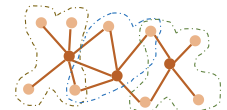
\includegraphics[width=2.30cm]{figures_zh/ch17/oa_generation}};
  \node at (3.11,19.04) {\#商业　\#体育　\#教育};
  \fill[orange!85!black] (2.02,18.72) circle (.045);
  \node[anchor=west,font=\fontsize{7}{8}\selectfont] at (2.11,18.72) {核心用户};
  \fill[orange!40] (3.25,18.72) circle (.045);
  \node[anchor=west,font=\fontsize{7}{8}\selectfont] at (3.34,18.72) {普通用户};
  \node[font=\fontsize{8}{9.2}\selectfont\bfseries] at (3.11,18.32) {大规模用户生成};
  \draw[workflow] (3.11,18.10) -- node[right] {注册} (3.11,16.94);

  \node[font=\fontsize{8}{9.2}\selectfont\bfseries,text=orange!80!black] (oa-env-overview) at (5.80,18.24) {环境服务器};
  \node[font=\fontsize{8}{9.2}\selectfont\bfseries,text=blue!60!black] (oa-rec-overview) at (8.51,18.24) {推荐系统};
  \node[font=\fontsize{8}{9.2}\selectfont\bfseries,text=yellow!40!black] (oa-agent-overview) at (10.96,18.24) {智能体};
  \node[font=\fontsize{8}{9.2}\selectfont\bfseries,text=green!40!black] (oa-time-overview) at (14.19,18.24) {时间引擎};
  \draw[workflow] (5.80,19.20) -- node[left] {注册} (oa-env-overview.north);
  \draw[workflow] (oa-env-overview.east) -- node[above,align=center,font=\fontsize{7}{8}\selectfont]
    {用户信息、帖子\\信息与关系} (oa-rec-overview.west);
  \draw[workflow] (oa-rec-overview.east) -- node[above,font=\fontsize{7}{8}\selectfont]
    {筛选后的帖子} (oa-agent-overview.west);
  \draw[workflow] (oa-agent-overview.north) -- (10.96,19.38) --
    node[above] {动作} (6.55,19.38) -- (oa-env-overview.north east);
  \draw[timeflow] (oa-time-overview.west) -- node[above] {激活} (oa-agent-overview.east);
  \draw[timeflow] (12.46,18.52) -- (12.46,20.25);
  \draw[green!40!black,thick] (12.27,19.25) -- (12.46,19.25);
  \draw[green!40!black,thick] (12.27,19.77) -- (12.46,19.77);
  \node[anchor=west,font=\fontsize{7}{8}\selectfont,text=green!40!black] at (12.53,19.25) {下午1时};
  \node[anchor=west,font=\fontsize{7}{8}\selectfont,text=green!40!black] at (12.53,19.77) {下午2时};
  \node[inner sep=0pt] at (14.34,19.75) {
\includegraphics[width=1.45cm]{figures_zh/ch17/oa_frequency}};
  \node[align=center,font=\fontsize{7.3}{8.3}\selectfont] at (14.32,19.00) {不同时段的\\交互频率};
  \draw[timeflow] (14.19,18.78) -- node[right,font=\fontsize{7}{8}\selectfont] {初始化} (oa-time-overview.north);

  \draw[module,orange!80!black] (.10,9.10) rectangle (6.68,16.94);
  \node[font=\small\bfseries,text=orange!80!black,fill=white] at (1.65,16.94) {环境服务器};
  \fill[card] (.28,13.65) rectangle (6.47,16.55);
  \node[anchor=west,text=orange!80!black,font=\bfseries] at (.49,16.22) {用户};
  \node[inner sep=0pt] at (1.10,14.93) {
\includegraphics[height=1.79cm]{figures_zh/ch17/oa_user_pair}};
  \node[align=left,anchor=west,text width=4.38cm] at (1.84,15.40) {姓名｜简介｜关注者列表……};
  \node[align=left,anchor=west,text width=4.38cm] at (1.84,14.51) {姓名｜简介｜关注者列表……};
  \node[anchor=west] at (.57,13.93) {$\cdots$};

  \fill[card] (.28,10.99) rectangle (6.47,13.36);
  \node[anchor=west,text=orange!80!black,font=\bfseries] at (.49,13.08) {帖子};
  \node[inner sep=0pt] at (.85,12.42) {
\includegraphics[width=.63cm]{figures_zh/ch17/oa_post1}};
  \node[anchor=west] at (1.31,12.42) {真不错……};
  \node[inner sep=0pt] at (4.87,12.42) {
\includegraphics[width=2.25cm]{figures_zh/ch17/oa_counts1}};
  \node[inner sep=0pt] at (.85,11.66) {
\includegraphics[width=.63cm]{figures_zh/ch17/oa_post2}};
  \node[anchor=west] at (1.31,11.66) {这是一个……};
  \node[inner sep=0pt] at (4.87,11.66) {
\includegraphics[width=2.25cm]{figures_zh/ch17/oa_counts2}};
  \node[anchor=west] at (.57,11.21) {$\cdots$};

  \fill[card] (.28,9.34) rectangle (6.47,10.74);
  \node[anchor=west,text=orange!80!black,font=\bfseries] at (.49,10.47) {动态智能体网络};
  \node[inner sep=0pt] at (1.26,9.86) {
\includegraphics[width=1.05cm]{figures_zh/ch17/oa_network_before_clean}};
  \node[inner sep=0pt] at (4.93,9.86) {
\includegraphics[width=1.05cm]{figures_zh/ch17/oa_network_after}};
  \draw[->,orange!80!black] (2.08,9.87) -- node[above] {更新} (4.10,9.87);
  \node[anchor=west] at (.57,9.16) {$\cdots$};

  \draw[module,blue!65] (8.19,9.10) rectangle (15.48,16.94);
  \node[font=\small\bfseries,text=blue!60!black,fill=white] at (10.08,16.94) {推荐系统};
  \draw[workflow] (6.68,15.13) -- node[above,font=\fontsize{7}{8}\selectfont,text=orange!80!black] {用户信息} (8.19,15.13);
  \draw[workflow] (6.68,12.34) -- node[above,font=\fontsize{7}{8}\selectfont,text=orange!80!black] {帖子信息} (8.19,12.34);
  \draw[workflow] (6.68,10.10) -- node[above,font=\fontsize{7}{8}\selectfont,text=orange!80!black] {关系} (8.19,10.10);
  \node[inner sep=0pt] at (9.88,15.02) {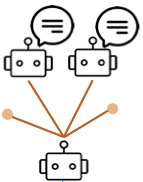
\includegraphics[height=2.75cm]{figures_zh/ch17/oa_rec_agents_clean}};
  \node[inner sep=0pt] at (13.65,15.46) {
\includegraphics[width=2.25cm]{figures_zh/ch17/oa_rec_pool}};
  \draw[recflow] (13.65,14.39) -- (13.65,14.11);
  \node[draw=blue!60!black,rounded corners=2pt,text=blue!60!black,minimum width=2.50cm,minimum height=.37cm]
    (oa-interest) at (13.65,13.87) {兴趣匹配};
  \draw[recflow] (oa-interest.south) -- (13.65,13.40);
  \draw[recflow] (9.88,13.62) -- (9.88,13.40);
  \draw[queue] (8.73,12.55) rectangle (11.03,13.38);
  \node[inner sep=0pt] at (9.88,12.96) {
\includegraphics[width=1.77cm]{figures_zh/ch17/oa_rec_in}};
  \node[text=blue!60!black,font=\bfseries] at (9.88,12.24) {网络内};
  \draw[queue] (12.50,12.55) rectangle (14.80,13.38);
  \node[inner sep=0pt] at (13.65,12.96) {
\includegraphics[width=1.77cm]{figures_zh/ch17/oa_rec_out}};
  \node[text=blue!60!black,font=\bfseries] at (13.65,12.24) {网络外};
  \draw[queue] (10.61,11.44) rectangle (12.91,12.26);
  \node[inner sep=0pt] at (11.76,11.85) {
\includegraphics[width=1.77cm]{figures_zh/ch17/oa_rec_hot}};
  \node[text=blue!60!black,font=\bfseries] at (11.76,11.20) {热度得分};
  \node[inner sep=0pt] at (11.76,10.10) {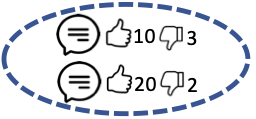
\includegraphics[width=3.50cm]{figures_zh/ch17/oa_rec_scores}};
  \draw[recflow] (11.76,10.91) -- (11.76,11.04);

  \draw[workflow] (11.76,9.10) -- (11.76,8.69) -- (3.73,8.69) -- (3.73,8.34);
  \node[fill=white] at (7.74,8.69) {筛选后的帖子};

  \draw[module,yellow!60!black] (.10,.50) rectangle (7.42,8.34);
  \node[font=\small\bfseries,text=yellow!40!black,fill=white] at (1.67,8.34) {智能体模块};
  \node[text=blue!60!black,font=\bfseries] at (2.77,7.76) {筛选帖子};
  \node[text=orange!80!black,font=\bfseries] at (5.00,7.76) {智能体信息};
  \draw[->,yellow!60!black] (3.73,7.49) -- (3.73,7.14);
  \node[inner sep=0pt] at (3.73,6.67) {
\includegraphics[width=1.02cm]{figures_zh/ch17/oa_memory}};
  \node[font=\bfseries,text=yellow!40!black] at (3.73,5.99) {记忆};
  \draw[->,yellow!60!black] (3.73,5.74) -- (3.73,5.40);
  \node[inner sep=0pt] at (2.70,4.89) {
\includegraphics[width=3.39cm]{figures_zh/ch17/oa_models_agent}};
  \node[inner sep=0pt] at (1.29,4.10) {
\includegraphics[width=.53cm]{figures_zh/ch17/oa_openai}};
  \node[font=\bfseries,text=yellow!40!black] at (2.18,4.10) {LLM};
  \draw[->,yellow!60!black] (3.73,4.29) -- (3.73,3.90);
  \node[align=center,font=\bfseries] at (1.30,3.38) {这真让我\\感兴趣！};
  \node[font=\bfseries,text=yellow!40!black] at (1.30,2.71) {理由};
  \draw[dashed,yellow!60!black,rounded corners=3pt] (3.00,2.50) rectangle (6.67,3.90);
  \node[inner sep=0pt] at (4.84,3.48) {
\includegraphics[width=3.08cm]{figures_zh/ch17/oa_actions}};
  \node[font=\fontsize{7.5}{8.5}\selectfont,text=yellow!40!black] at (3.68,2.86) {发帖};
  \node[font=\fontsize{7.5}{8.5}\selectfont,text=yellow!40!black] at (4.46,2.86) {点赞};
  \node[font=\fontsize{7.5}{8.5}\selectfont,text=yellow!40!black] at (5.45,2.86) {评论};
  \node[font=\bfseries,text=yellow!40!black] at (4.84,2.15) {动作};
  \draw[workflow] (4.84,1.85) -- (4.84,1.34);
  \node[font=\bfseries,text=orange!80!black] at (4.84,.94) {环境服务器};
  \node[inner sep=0pt] at (1.87,1.05) {
\includegraphics[width=2.69cm]{figures_zh/ch17/oa_logo}};

  \draw[module,green!35!black] (8.19,4.47) rectangle (15.48,8.34);
  \node[font=\small\bfseries,text=green!35!black,fill=white] at (9.74,8.34) {时间引擎};
  \draw[timeflow] (9.48,5.15) -- (9.48,7.91);
  \draw[green!40!black] (9.32,7.31) -- (9.48,7.31);
  \fill[green!40!black] (9.48,5.91) circle (.08);
  \node[anchor=east,text=green!40!black] at (9.21,7.31) {下午2时};
  \node[anchor=east,text=green!40!black] at (9.21,5.91) {下午1时};
  \node[inner sep=0pt] at (8.92,5.18) {
\includegraphics[width=.50cm]{figures_zh/ch17/oa_clock}};
  \node[inner sep=0pt] at (12.67,6.71) {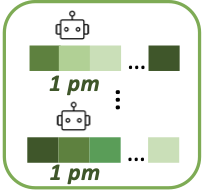
\includegraphics[width=3.15cm]{figures_zh/ch17/oa_time_queues}};
  \fill[white] (11.73,6.68) rectangle (12.96,7.10);
  \node[text=green!35!black] at (12.34,6.89) {下午1时};
  \fill[white] (11.73,5.28) rectangle (12.96,5.72);
  \node[text=green!35!black] at (12.34,5.50) {下午1时};
  \node[inner sep=0pt] at (12.67,4.73) {
\includegraphics[width=3.50cm]{figures_zh/ch17/oa_active_bar_clean}};
  \node[font=\bfseries] at (12.71,4.73) {活跃程度};
  \draw[timeflow] (8.19,6.05) -- node[above,sloped,fill=white] {激活} (4.35,4.98);

  \draw[module,gray] (8.19,.50) rectangle (15.48,3.96);
  \node[font=\small\bfseries,text=gray,fill=white] at (10.41,3.96) {可扩展推理器};
  \node[inner sep=0pt] at (11.83,2.23) {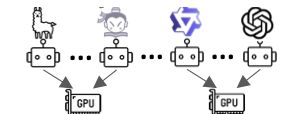
\includegraphics[width=6.52cm]{figures_zh/ch17/oa_inferencer_clean}};
  \draw[->,gray,line width=.8pt] (12.41,.87) -- (13.87,.87);
  \node[text=gray,anchor=west] at (14.04,.87) {线程};
  \draw[->,gray,line width=1.15pt] (4.35,4.71) --
    node[above,sloped,fill=white] {推理} (7.82,4.22) -- (8.19,2.55);
\end{tikzpicture}
